%%%%%%%%%%%%%%%%%%%%%%%%%%%%%%%%%%%%%%%%%
% NIWeek 2014 Poster by T. Reveyrand
% www.microwave.fr
% http://www.microwave.fr/LaTeX.html
% ---------------------------------------
% 
% Original template created by:
% Brian Amberg (baposter@brian-amberg.de)
%
% This template has been downloaded from:
% http://www.LaTeXTemplates.com
%
% License:
% CC BY-NC-SA 3.0 (http://creativecommons.org/licenses/by-nc-sa/3.0/)
%
%%%%%%%%%%%%%%%%%%%%%%%%%%%%%%%%%%%%%%%%%

%----------------------------------------------------------------------------------------
%   PACKAGES AND OTHER DOCUMENT CONFIGURATIONS
%----------------------------------------------------------------------------------------

\documentclass[b1paper,portrait]{baposter}

\usepackage[font=small,labelfont=bf]{caption} % Required for specifying captions to tables and figures
\usepackage{booktabs} % Horizontal rules in tables
\usepackage{relsize} % Used for making text smaller in some places

\usepackage{amsmath,amsfonts,amssymb,amsthm} % Math packages
\usepackage{eqparbox}

\usepackage{textcomp}

\usepackage{caption}
\usepackage{subcaption}
\usepackage{graphicx}
%\usepackage{hyperref}

\graphicspath{{figures/}} % Directory in which figures are stored

 \definecolor{bordercol}{RGB}{40,40,40} % Border color of content boxes
 \definecolor{headercol1}{RGB}{186,215,230} % Background color for the header in the content boxes (left side)
 \definecolor{headercol2}{RGB}{120,120,120} % Background color for the header in the content boxes (right side)
 \definecolor{headerfontcol}{RGB}{0,0,0} % Text color for the header text in the content boxes
 \definecolor{boxcolor}{RGB}{210,235,250} % Background color for the content in the content boxes


\begin{document}

\background{ % Set the background to an image (background.pdf)
\begin{tikzpicture}[remember picture,overlay]
\draw (current page.north west)+(-2em,2em) node[anchor=north west]
{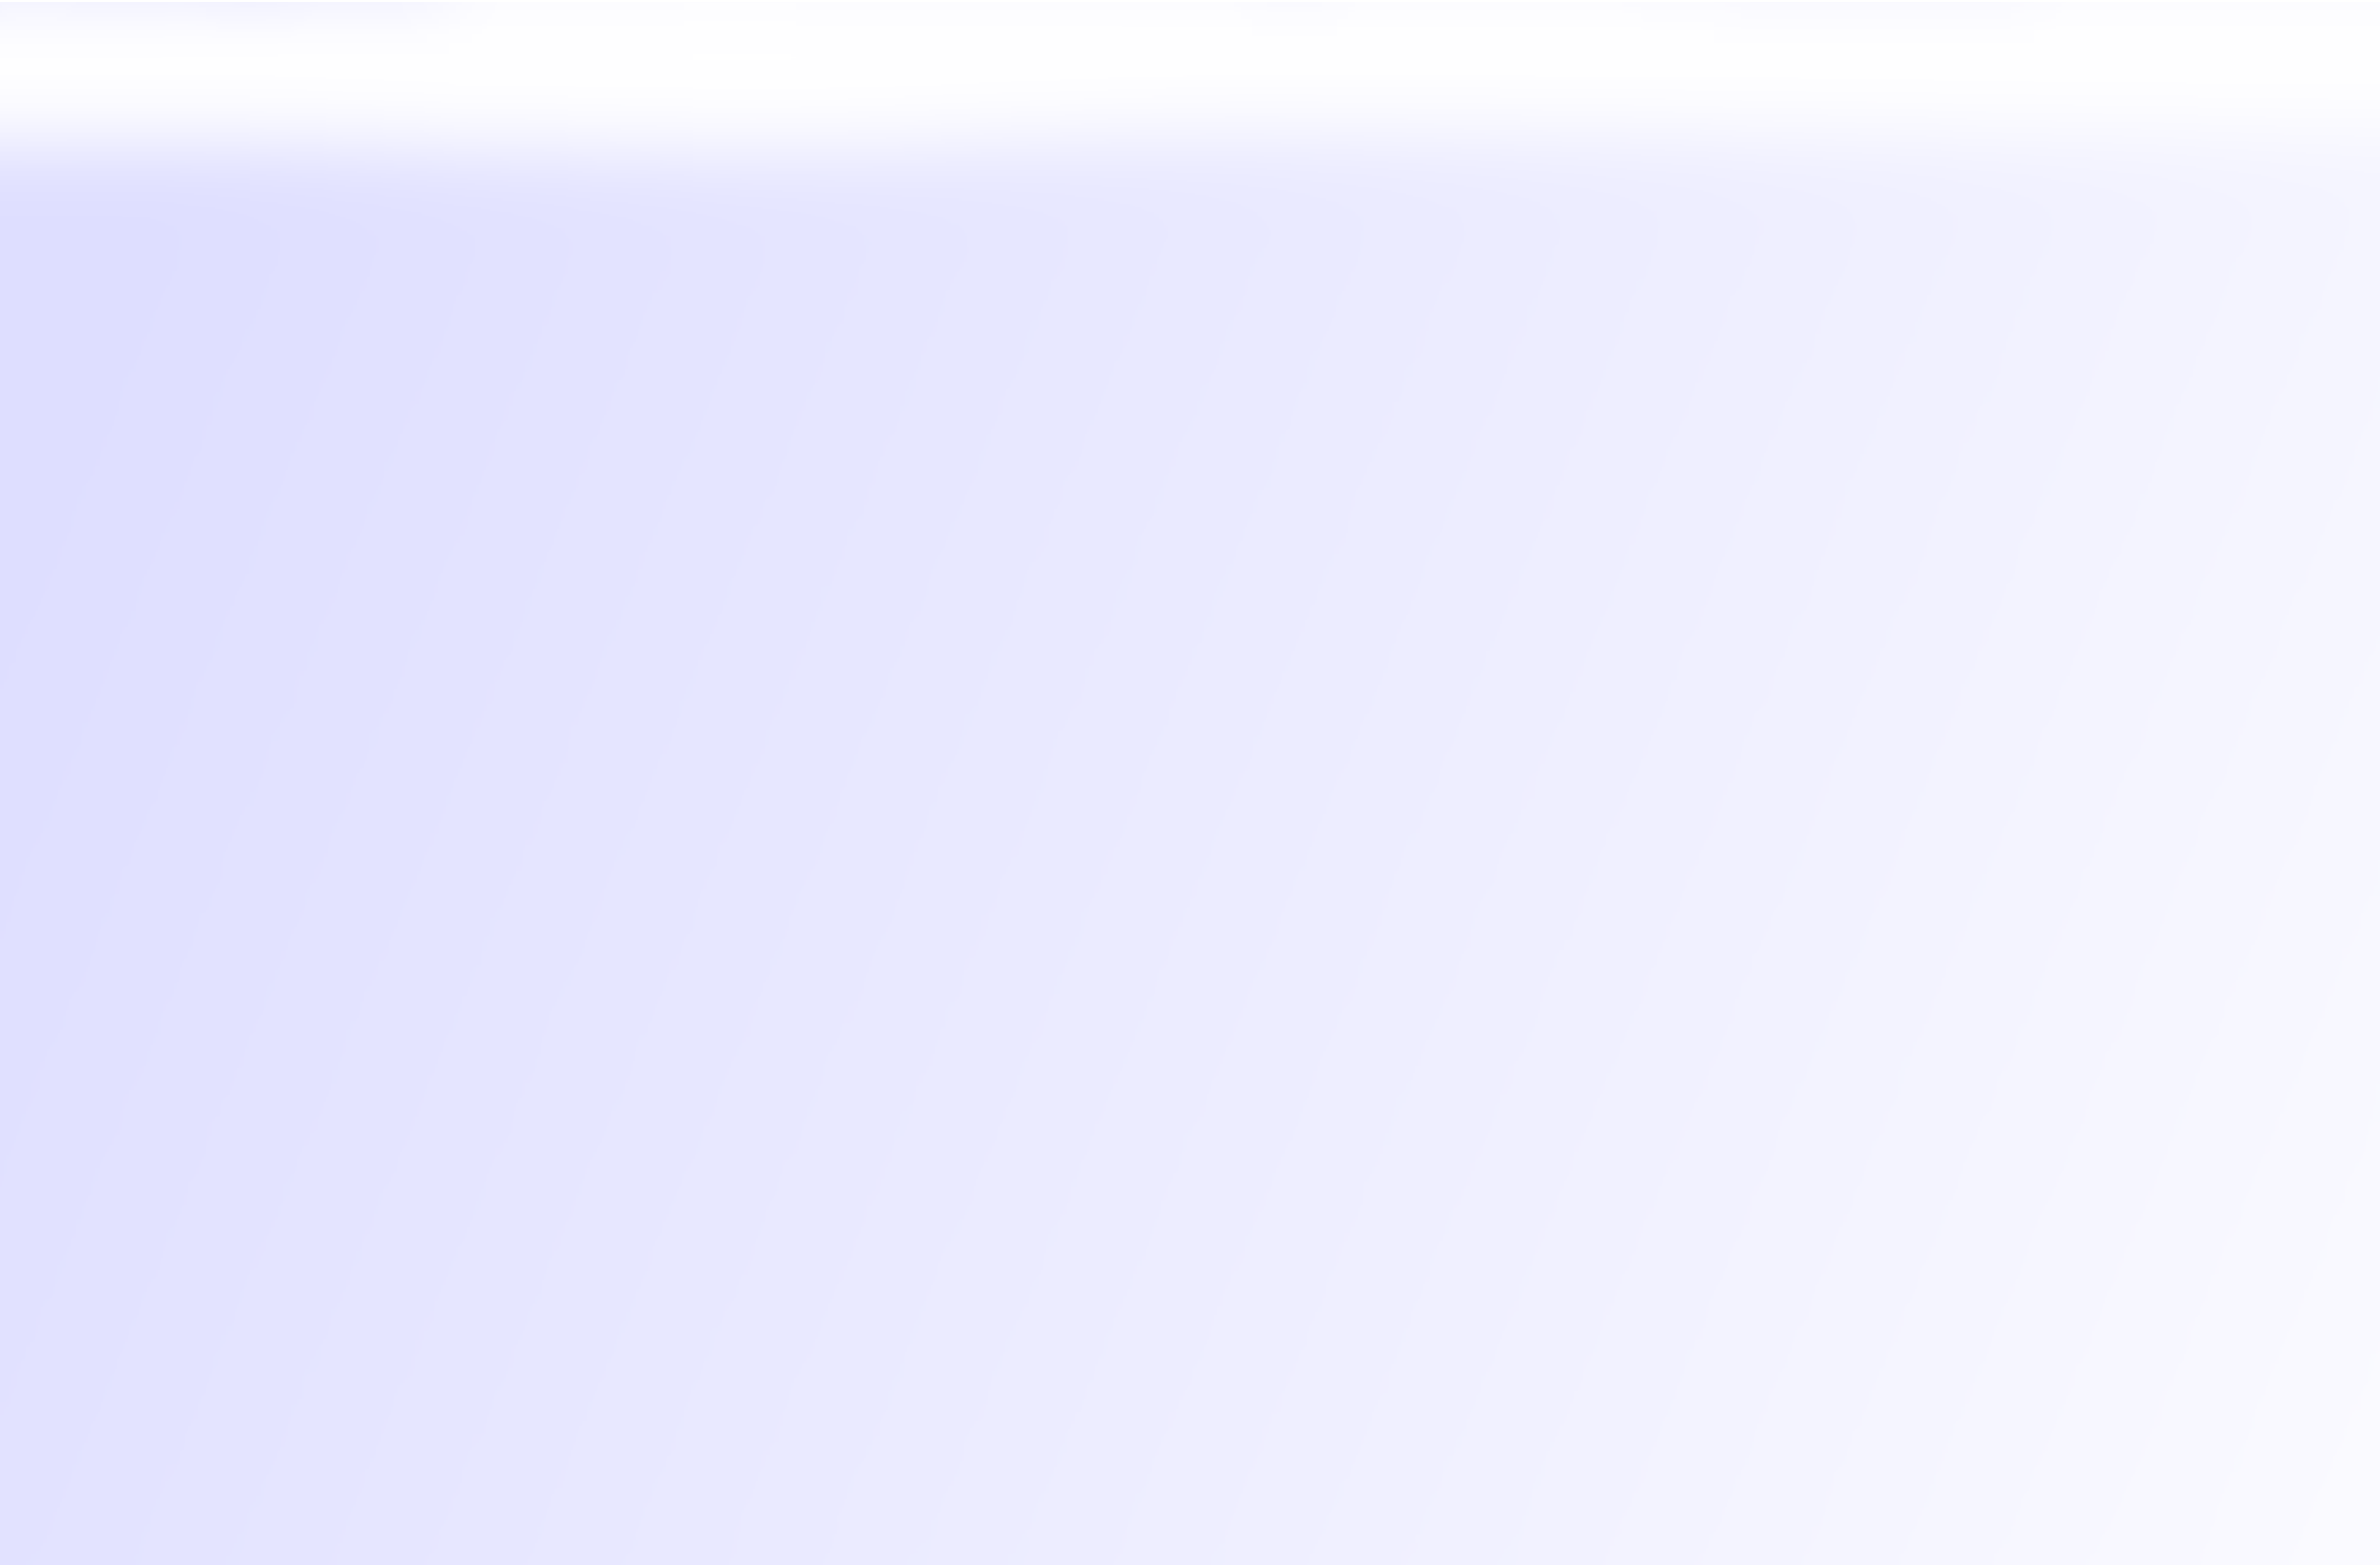
\includegraphics[height=1.1\textheight]{background}};
\end{tikzpicture}
}

\begin{poster}{
grid=false,
columns=4,
borderColor=bordercol, % Border color of content boxes
headerColorOne=headercol1, % Background color for the header in the content boxes (left side)
headerColorTwo=headercol2, % Background color for the header in the content boxes (right side)
headerFontColor=headerfontcol, % Text color for the header text in the content boxes
boxColorOne=boxcolor, % Background color for the content in the content boxes
headershape=roundedright, % Specify the rounded corner in the content box headers
headerfont=\Large\sf\bf, % Font modifiers for the text in the content box headers
textborder=rectangle,
background=none,
headerborder=open, % Change to closed for a line under the content box headers
boxshade=plain
}
{
\includegraphics[width=3.5cm]{sigmod_2018.png}}
%
%----------------------------------------------------------------------------------------
%   TITLE AND AUTHOR NAME
%----------------------------------------------------------------------------------------
%
{ \bf  \huge {CFPQ by Matrix Multiplication} \\  \Large \it Matrix-based algorithm for graph structured data analysis} % Poster title
{\vspace{0.3em} \smaller Rustam Azimov$^1$, Semyon Grigorev$^1$,  \\  % Author names
\smaller \it $^1${Saint Petersburg State University, JetBrains, St. Petersburg, Russia } \\ % Author email addresses
\smaller  {\textbf{E-mails:} st013567@student.spbu.ru, s.v.grigoriev@spbu.ru}}
{
\includegraphics[width=2cm]{SPbGU_Logo.png}} % University/lab logo


%----------------------------------------------------------------------------------------
%   INTRODUCTION
%----------------------------------------------------------------------------------------
\headerbox{Motivation}{name=introduction,column=0,row=0, span=2}{
Context-free path querying (CFPQ) is a technique, which recently gains popularity in graph databases, bioinformatics, static analysis, etc. It is often required to query large graphs, and existing algorithms demonstrate a poor performance in this case. We propose the first generalization of matrix-based Valiant's algorithm for context-free path querying. The utilization of matrix operations in the process of context-free path query evaluation makes it possible to efficiently apply a wide class of optimizations and computing techniques for querying large graphs, such as GPGPU, parallel processing, sparse matrix representation, distributed-memory computation, etc.
}

\headerbox{Results}{name=results,column=2,row=0, span=2}{
\begin{itemize} 
\item We propose the matrix-based algorithm for context-free path querying.
\vspace{-0.2cm}
\item We implemented this algorithm with a number of optimizations (sparse matrix representation, GPGPU) and applied this implementation to the navigation query problem for some popular RDF ontologies, taken from~\cite{RDF}.
\vspace{-0.2cm}
\item We also compared the performance of our implementation with the fastest analog from~\cite{GLL} (based on GLL).
\vspace{-0.6cm}
\item All materials are available on GitHub: \small{https://github.com/YaccConstructor}
\end{itemize}
}

\headerbox{Evaluation}{name=eval,column=2,row=0, span=2, below=results}{	
	\begin{center}		
		Evaluation results for the query $S \rightarrow aSb|cSd|ab|cd$ for retrieving the concepts on the same layer.
		
		\begin{tabular}{ | c | c | c | c | c |}
			\hline
			Ontology & V & E & GLL\cite{GLL}(ms)& sGPU(ms)\\
			\hline 
			\hline
			%		skos        & 144 & 323 & 10 & 12\\
			%		generations & 129 & 351 & 19 & 13\\
			%		travel      & 131 & 397 & 24 & 30\\
			%		univ-bench  & 179 & 413 & 25 & 15\\
			%		atom-primitive & 291 & 685 & 255 & 22\\
			biomedical & 341 & 711 & 261 & 20\\
			%		foaf        & 256 & 815 & 48 & 9\\
			people-pets & 337 & 834 & 89 & 32\\
			%		funding     & 778 & 1480 & 212 & 36\\
			%		wine        & 733 & 2450 & 819 & 54\\
			pizza       & 671 & 2604 & 697 & 24\\
			$g_{1}$     & 6224 & 11840 & 1926 & 82\\
			$g_{2}$     & 5864 & 19600 & 6246 & 185\\
			$g_{3}$     & 5368 & 20832 & 7014 & 127\\
			\hline
		\end{tabular}
	
	\vspace{0.6cm}
		
		Evaluation results for the query $S \rightarrow Bb|b$ , $B \rightarrow aBb|ab$ for retrieving concepts on the adjacent layers.
		\begin{tabular}{ | c | c | c | c | c |}
			\hline
			Ontology & V & E & GLL\cite{GLL}(ms) & sGPU(ms)\\
			\hline 
			\hline
			%	skos        & 144 & 323 & 1 & 1\\
			%	generations & 129 & 351 & 1 & 0\\
			%	travel      & 131 & 397 & 1 & 10\\
			%	univ-bench  & 179 & 413 & 11 & 9\\
			%	atom-primitive & 291 & 685 & 66 & 2\\
			%	biomedical & 341 & 711 & 45 & 24\\
			%	foaf        & 256 & 815 & 2 & 3\\
			%	people-pets & 337 & 834 & 3 & 6\\
			funding     & 778 & 1480 & 23 & 27\\
			wine        & 733 & 2450 & 8 & 6\\
			pizza       & 671 & 2604 & 29 & 23\\
			$g_{1}$     & 6224 & 11840 & 167 & 38\\
			$g_{2}$     & 5864 & 19600 & 46 & 21\\
			$g_{3}$     & 5368 & 20832 & 393 & 40\\
			\hline
		\end{tabular}
	\end{center}
\vspace{0.2cm}
}
    
\headerbox{Future Research}{name=future,column=2,below=eval, span=2}{
 Currently, we are working on the matrix-based algorithm for path querying with conjunctive grammars which have more expressive power, than context-free grammars. We want to find new applications for the path querying techniques and implement the required tools.
}

\headerbox{Context-free path querying}{name=CFParsing,span=2,column=0,row=1,below=introduction}{
\begin{center}
	\textbf{The input edge-labeled directed graph}	
	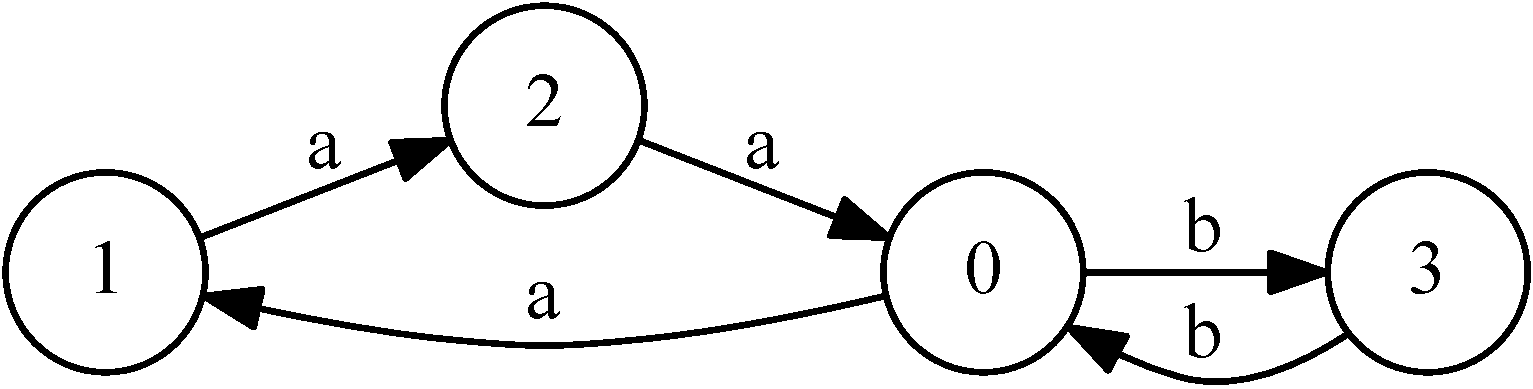
\includegraphics[width=7cm]{example_graph_transparent.png}
	
	\textbf{The input CF grammar for the language $L=\{a^n b^n\}$}	
	$\begin{array}{rcclrccl}
	0: & S & \rightarrow & A \ B & 3: & A & \rightarrow & \text{\emph{a}} \\  
	1: & S & \rightarrow & A \ S_1 & 4: & B & \rightarrow & \text{\emph{b}} \\
	2: & S_1 & \rightarrow & S \ B & & & & \\
	
	\end{array}$
\end{center}

The result is a set of node pairs corresponding to paths, whose labeling is in the input language $L$.
}

\headerbox{Matrix-based approach}
{name=app1,column=0,span=2, below=CFParsing}
{ % To reduce this block to 1 column width, remove 'span=2'
	We compute the following matrix transitive closure:
	$$T^{(i)} = T^{(i-1)} \cup (T^{(i-1)} \times T^{(i-1)}), ~i \ge 1.$$ 
	\begin{center}
	\textbf{The initial adjacency matrix for the input graph}
	\[
	T_0 = \begin{pmatrix}
		\varnothing & \{A\}       & \varnothing & \{B\}       \\
		\varnothing & \varnothing & \{A\}       & \varnothing \\
		\{A\}       & \varnothing & \varnothing & \varnothing \\
		\{B\}       & \varnothing & \varnothing & \varnothing \\
	\end{pmatrix}
	\]
	\textbf{The first iteration}
	\[
	T_1 = T_0 \cup (T_0 \times T_0) = \begin{pmatrix}
	\varnothing & \{A\}       & \varnothing & \{B\}       \\
	\varnothing & \varnothing & \{A\}       & \varnothing \\
	\{A\}       & \varnothing & \varnothing & \{\pmb{S}\}       \\
	\{B\}       & \varnothing & \varnothing & \varnothing \\
	\end{pmatrix}
	\]
	\textbf{The final matrix}
	\[
	T_{13} = \begin{pmatrix}
		\{S_1, S\}     & \{A\}       & \varnothing & \{B, S, S_1\}    \\
		\{S, S_1\}       & \varnothing & \{A\}       & \{S_1, S\}     \\
		\{A, S_1, S\}  & \varnothing & \varnothing & \{S, S_1\} \\
		\{B\}       & \varnothing & \varnothing & \varnothing \\
	\end{pmatrix}
	\]
	\end{center}

The indices of the elements of $T_{13}$ which contain the non-terminal $S$ are node pairs corresponding to paths, whose labeling is in the given language $\{a^n b^n\}$.
\vspace{0.44cm}
}


\headerbox{Acknowledgments}{name=ack,column=2,below=future, span=2}{
The research was supported by the Russian Science Foundation grant 18-11-00100 and a grant from JetBrains Research.
}

%----------------------------------------------------------------------------------------
%   REFERENCES
%----------------------------------------------------------------------------------------

\headerbox{References}{name=references,column=2,span=2,below=ack}{
	
	\smaller % Reduce the font size in this block
	\renewcommand{\section}[2]{\vskip 0.05em} % Get rid of the default "References" section title
	%\nocite{*} % Insert publications even if they are not cited in the poster
	
	\bibliographystyle{unsrt}
	\bibliographystyle{IEEEtran}
	\bibliography{biblio} % Use biblio.bib as the bibliography file
}



\end{poster}

\end{document}